\documentclass[12pt,letterpaper]{article}
\usepackage{graphicx,textcomp}
\usepackage{natbib}
\usepackage{setspace}
\usepackage{fullpage}
\usepackage{color}
\usepackage[reqno]{amsmath}
\usepackage{amsthm}
\usepackage{fancyvrb}
\usepackage{amssymb,enumerate}
\usepackage[all]{xy}
\usepackage{endnotes}
\usepackage{lscape}
\newtheorem{com}{Comment}
\usepackage{float}
\usepackage{hyperref}
\newtheorem{lem} {Lemma}
\newtheorem{prop}{Proposition}
\newtheorem{thm}{Theorem}
\newtheorem{defn}{Definition}
\newtheorem{cor}{Corollary}
\newtheorem{obs}{Observation}
\usepackage[compact]{titlesec}
\usepackage{dcolumn}
\usepackage{tikz}
\usetikzlibrary{arrows}
\usepackage{multirow}
\usepackage{xcolor}
\newcolumntype{.}{D{.}{.}{-1}}
\newcolumntype{d}[1]{D{.}{.}{#1}}
\definecolor{light-gray}{gray}{0.65}
\usepackage{url}
\usepackage{listings}
\usepackage{color}

\definecolor{codegreen}{rgb}{0,0.6,0}
\definecolor{codegray}{rgb}{0.5,0.5,0.5}
\definecolor{codepurple}{rgb}{0.58,0,0.82}
\definecolor{backcolour}{rgb}{0.95,0.95,0.92}

\lstdefinestyle{mystyle}{
	backgroundcolor=\color{backcolour},   
	commentstyle=\color{codegreen},
	keywordstyle=\color{magenta},
	numberstyle=\tiny\color{codegray},
	stringstyle=\color{codepurple},
	basicstyle=\footnotesize,
	breakatwhitespace=false,         
	breaklines=true,                 
	captionpos=b,                    
	keepspaces=true,                 
	numbers=left,                    
	numbersep=5pt,                  
	showspaces=false,                
	showstringspaces=false,
	showtabs=false,                  
	tabsize=2
}
\lstset{style=mystyle}
\newcommand{\Sref}[1]{Section~\ref{#1}}
\newtheorem{hyp}{Hypothesis}

\setcounter{secnumdepth}{0}

\title{Problem Set 1}
\author{Applied Stats/Quant Methods 1}
\date{Due: October 8, 2026}
\author{Barrera Munoz Diego}

\begin{document}
	\maketitle
	\tableofcontents
	\newpage

	\section{Question 1: Education}

A school counselor was curious about the average of IQ of the students in her school and took a random sample of 25 students' IQ scores. The following is the data set:\\

\lstinputlisting[language=R, firstline=37, lastline=37]{PS01.R}  

\begin{enumerate}
	
	% Question 1.1:
	\item Find a 90\% confidence interval for the average student IQ in the school (As a hint, you first need the mean and SD to create a CI):\\
	
\vspace{.5cm}
	
\textbf{Answer:} Since we don't know the population standard deviation ($\sigma$), and the size of our sample is small, we will be working with a $t$ distribution to create a CI. 

First, we need to calculate the sample size ($n$), sample mean ($\bar{y}$), standard deviation ($s$) and the standard error ($SE$). 

$$SE = \frac{s}{\sqrt{n}}$$

\lstinputlisting[language=R, firstline=41, lastline=47]{PS01.R}

\begin{verbatim}
 'y' has 25 observations, 
The sample mean is : 98.44  
The standard deviation is:  13.09287  
And the standard error is:  2.618575
\end{verbatim}

Then we need to calculate the critical value ($t$). We can use this R code:

\lstinputlisting[language=R, firstline=49, lastline=50]{PS01.R}

\begin{verbatim}
[1] 1.710882
\end{verbatim}

Note that we use $p = 0.95$ in the code because we want $5\%$ in the lower tail and $5\%$ in the upper tail, leaving $90\%$ in the centre of the distribution.

Then the $90\%$ CI will be:

$$CI = \bar{y} \pm t(SE)$$
$$CI_{90\%} = 98.44 \pm 1.710882(2.618575) = [93.96,\ 102.92]$$

The CI can also be obtained with this R code:

\lstinputlisting[language=R, firstline=52, lastline=54]{PS01.R}

\begin{verbatim}
 Lower  Upper 
93.96 102.92 
\end{verbatim}

In repeated random sampling, about $90\%$ of intervals made this way
would contain the true school mean.

\

	% Question 1.2:
	\item Next, the school counselor was curious  whether  the average student IQ in her school is higher than the average IQ score (100) among all the schools in the country.\\ 
	
	\noindent Using the same sample, conduct the appropriate hypothesis test with $\alpha=0.05$.
	
\vspace{.5cm}
	
\textbf{Answer:} To perform an appropriate hypothesis test, first we need to examine the data and formulate the hypotheses. The sample is small, the students were selected randomly, and IQ scores are measured on an interval scale. The school counselor wants to test whether the average IQ score is greater than 100. Therefore, our null and alternative hypotheses are:

\begin{itemize}
	\item $H_0 \colon \mu \leq 100$
	\item $H_a \colon \mu > 100$  
\end{itemize}

Then, for the test statistic, we will use a right-tailed, one-sample $t$-test because we want to test whether the population mean $\mu$ is \emph{higher} than 100:

$$t = \frac{\bar{y} - \mu_0}{SE}$$

$$t = \frac{98.44 - 100}{2.618575} = -0.5957$$

\vspace{.5cm}

For a one-sided test with $\alpha = 0.05$ and $df = 24$:

$$t_{0.95, 24} \approx 1.711$$

Since $-1.711 < -0.5957 < 1.711$ we \textbf{fail to reject the null hypothesis} and therefore there is not enough evidence that the school's mean IQ is greater than $100$ (with an $\alpha = 0.05$).

\vspace{.5cm}

We can verify our results with this R code:

\lstinputlisting[language=R, firstline=58, lastline=58]{PS01.R}

\begin{verbatim}
	One Sample t-test

data:  y
t = -0.59574, df = 24, p-value = 0.7215
alternative hypothesis: true mean is greater than 100
95 percent confidence interval:
93.95993      Inf
sample estimates:
mean of x 
98.44 
\end{verbatim}

With this code we can observe that the p-value is $0.7215$.

Since $0.7215$ is not less than $0.05$ ($\alpha$ value), we fail to reject the null hypothesis.

\end{enumerate}

\newpage

	\section{Question 2: Political Economy}

\noindent Researchers are curious about what affects the amount of money communities spend on addressing homelessness. The following variables constitute our data set about social welfare expenditures in the USA. \\
\vspace{.5cm}


\begin{tabular}{r|l}
	\texttt{State} &\emph{50 states in US} \\
	\texttt{Y} & \emph{per capita expenditure on shelters/housing assistance in state}\\
	\texttt{X1} &\emph{per capita personal income in state} \\
	\texttt{X2} &  \emph{Number of residents per 100,000 that are "financially insecure" in state}\\
	\texttt{X3} &  \emph{Number of people per thousand residing in urban areas in state} \\
	\texttt{Region} &  \emph{1=Northeast, 2= North Central, 3= South, 4=West} \\
\end{tabular}

\vspace{.5cm}
\noindent Explore the \texttt{expenditure} data set and import data into  \texttt{R}. %Question 2.1
\vspace{.5cm}
\lstinputlisting[language=R, firstline=64, lastline=64]{PS01.R}  

\noindent \textbf{Answer:} First, we need to look at the structure of the data and check whether the data set contains any missing values (NAs):

\lstinputlisting[language=R, firstline=68, lastline=70]{PS01.R}

\begin{verbatim}
> print(head(expenditure))
STATE  Y   X1  X2  X3 Region
1    ME 61 1704 388 399      1
2    NH 68 1885 272 598      1
3    VT 72 1745 397 370      1
4    MA 72 2394 458 868      1
5    RI 62 1966 157 899      1
6    CT 91 2817 162 690      1
> print(dim(expenditure))
[1] 50  6
> print(sum(is.na(expenditure)))
[1] 0
\end{verbatim}

\noindent The data contain 50 states (rows), six columns and no missing values (NAs).

\vspace{.5cm}
\begin{itemize}

\item
Please plot the relationships among \emph{Y}, \emph{X1}, \emph{X2}, and \emph{X3}? What are the correlations among them (you just need to describe the graph and the relationships among them)? % Question 2.2
\vspace{.5cm}

\textbf{Answer:} We can use a scatterplot matrix to compare every pair of
numerical variables with this R code:

\lstinputlisting[language=R, firstline=79, lastline=83]{PS01.R}

\begin{center}
	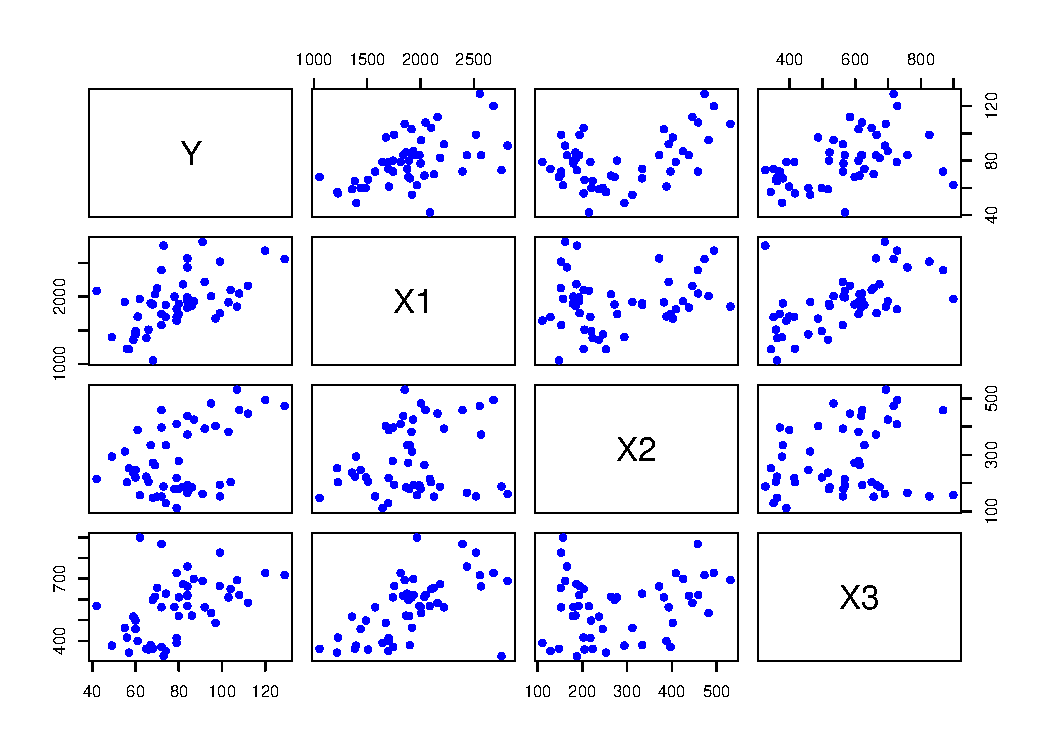
\includegraphics[width=\linewidth]{PS01_figures/scatterplot_matrix.pdf}
\end{center}

With this graph we can observe each variable plotted against the other ones, showing the relationships between six distinct pairs of variables. Some pairs of variables, including $X1$–$X3$ and $Y$–$X1$, appear to have moderate positive correlations. But if we want to better understand their relationships, we need to calculate the correlation coefficient for each pair of variables. We can use this R code for the calculation:

\newpage

\lstinputlisting[language=R, firstline=85, lastline=86]{PS01.R}

\begin{verbatim}
       Y    X1    X2    X3
Y  1.000 0.532 0.448 0.464
X1 0.532 1.000 0.206 0.595
X2 0.448 0.206 1.000 0.221
X3 0.464 0.595 0.221 1.000
\end{verbatim}

With this table we can observe that $Y$ (spending) has a moderate positive relationship with $X1$ (income), $X2$ (financial insecurity), and $X3$ (urbanisation). States with higher values of these variables tend to spend more, although the dots are quite spread out and therefore harder to fit into a linear regression model.

$X1$ and $X3$ have the strongest relationship of the six
($r=0.595$): higher-income states tend to be more urban. $X1$ and
$X2$ ($r=0.206$), and $X2$ and
$X3$ ($r=0.221$), have weak positive relationships.

These are associations; correlation does not establish causation.

\vspace{.5cm}
\item
Please plot the relationship between \emph{Y} and \emph{Region}? On average, which region has the highest per capita expenditure on housing assistance? % Question 2.3
\vspace{.5cm}

\textbf{Answer:} Since \emph{Region} is a categorical variable, we will use a boxplot to compare spending across the four groups. First, we need to create a factor variable, \emph{Region\_name}, from \emph{Region}, which is currently coded using the numbers $1$ to $4$.

\lstinputlisting[language=R, firstline=90, lastline=95]{PS01.R}

Then we create the boxplot:

\lstinputlisting[language=R, firstline=97, lastline=106]{PS01.R}

\begin{center}
	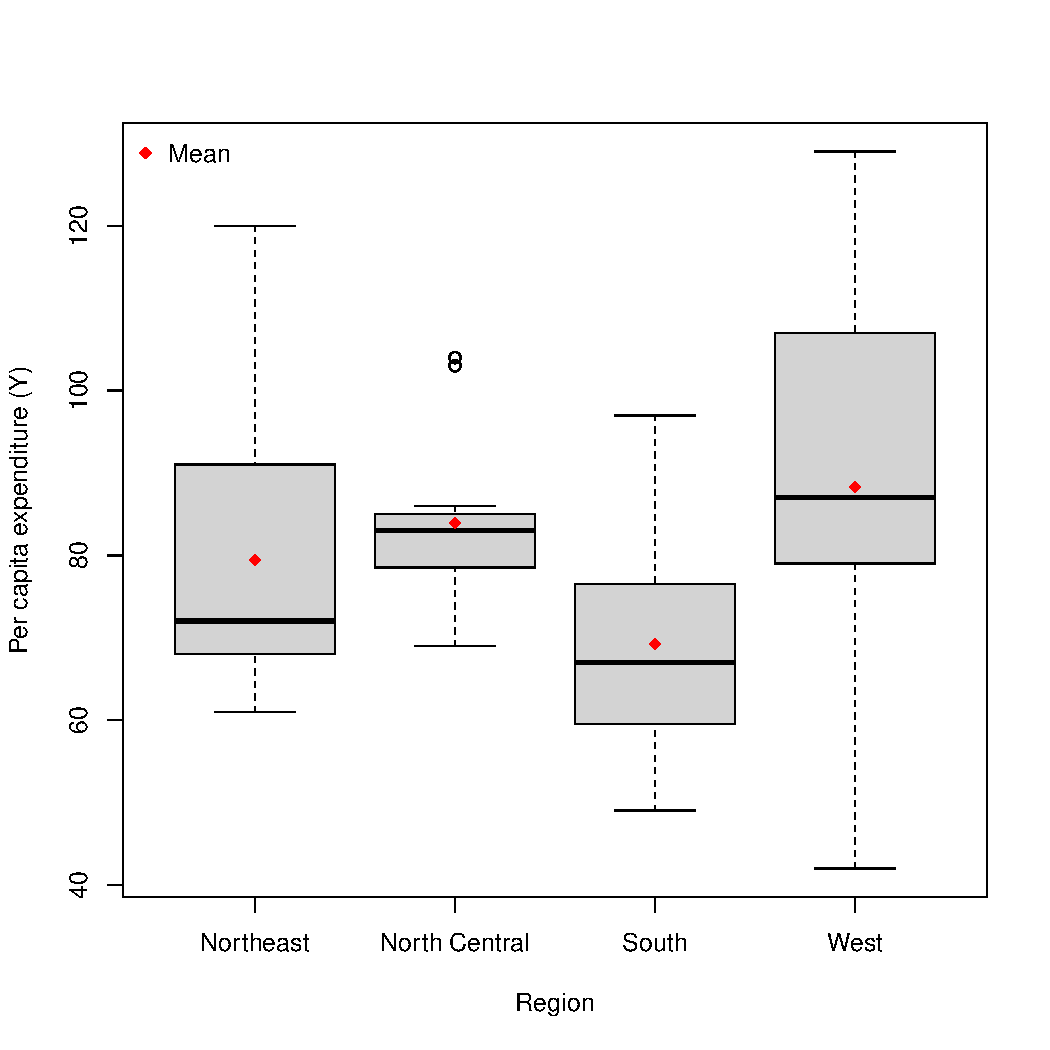
\includegraphics[width=0.88\linewidth,trim=0 0.1in 0 0.5in,clip]{PS01_figures/spending_by_region.pdf}
\end{center}

\lstinputlisting[language=R, firstline=108, lastline=108]{PS01.R}

\begin{verbatim}
    Northeast 			North Central       South        West 
				79.44        83.92         						69.19        88.31 
\end{verbatim}

The \textbf{West} region has the highest average expenditure, at $88.31$. The South region has the lowest, at $69.19$. The wide spread in the West indicates that spending varies considerably across its states, particularly compared with the North Central region, which has the second-highest average expenditure.

\newpage
\item
Please plot the relationship between \emph{Y} and \emph{X1}? Describe this graph and the relationship. Reproduce the above graph including one more variable \emph{Region} and display different regions with different types of symbols and colors. %Question 2.4

\textbf{Answer:} To create this plot, we will use the \emph{ggplot2} package:

\lstinputlisting[language=R, firstline=2, lastline=2]{PS01.R}

First, we put $X1$ (Income) on the horizontal axis and $Y$ (Spending)
on the vertical axis with this R code:

\lstinputlisting[language=R, firstline=112, lastline=118]{PS01.R}

\begin{center}
	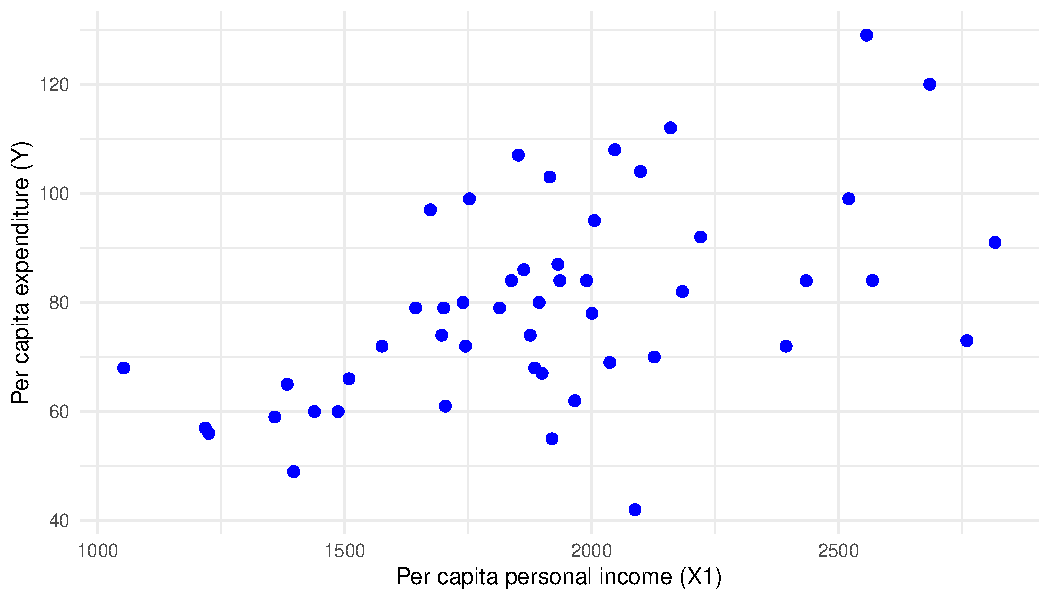
\includegraphics[width=\linewidth]{PS01_figures/spending_and_income.pdf}
\end{center}

We can observe that there is a \textbf{moderate positive relationship} ($r=0.532$). States with higher per capita income tend to spend more per person on housing assistance. Income and spending are positively associated, but states with similar incomes can have different spending levels.

\newpage
\textbf{Adding Region to the same graph:}

First, we use the mapping \emph{Region\_name} $\to$ colour and shape inside \emph{aes}(). Different shapes make the regions easier to distinguish. Then we select four different colours and shapes. Thus, the R code that produces the new plot is: 

\lstinputlisting[language=R, firstline=124, lastline=133]{PS01.R}

\begin{center}
	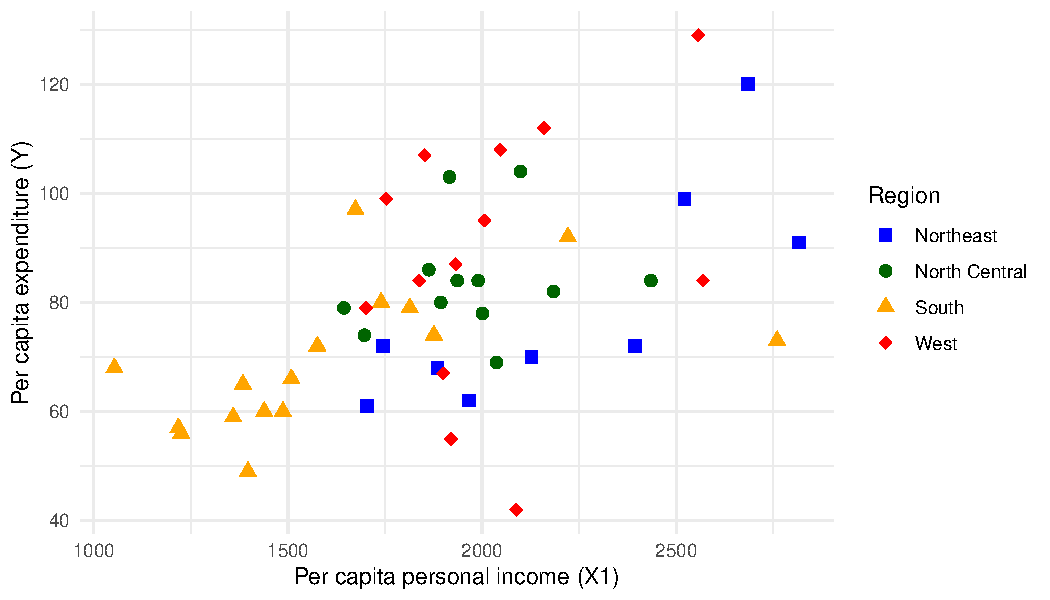
\includegraphics[width=\linewidth]{PS01_figures/income_and_spending_by_region.pdf}
\end{center}

With the updated plot we can observe that many Southern states (orange triangles) are in the lower-income, lower-spending part of the graph. Western states (red diamonds) have a wide spread in spending, including the lowest and highest values. 

Note that the groups overlap, so  \emph{Region} does not fully explain the  relationship.

\end{itemize}


\end{document}
